%%%%%%%%%%%%%%%%%%%%%%%%%%%%%%%%%%%%%%%%%
% University/School Laboratory Report
% LaTeX Template
% Version 3.1 (25/3/14)
%
% This template has been downloaded from:
% http://www.LaTeXTemplates.com
%
% Original author:
% Linux and Unix Users Group at Virginia Tech Wiki 
% (https://vtluug.org/wiki/Example_LaTeX_chem_lab_report)
%
% License:
% CC BY-NC-SA 3.0 (http://creativecommons.org/licenses/by-nc-sa/3.0/)
%
%%%%%%%%%%%%%%%%%%%%%%%%%%%%%%%%%%%%%%%%%

%----------------------------------------------------------------------------------------
%	PACKAGES AND DOCUMENT CONFIGURATIONS
%----------------------------------------------------------------------------------------

\documentclass{article}

\usepackage{graphicx} % Required for the inclusion of images
\usepackage{amsmath} % Required for some math elements 
%\usepackage{cite}
%\usepackage{subcaption} %Required to group figures
%\usepackage{float}

\setlength\parindent{0pt} % Removes all indentation from paragraphs

%\usepackage{times} % Uncomment to use the Times New Roman font

%----------------------------------------------------------------------------------------
%	DOCUMENT INFORMATION
%----------------------------------------------------------------------------------------

\title{Lab 4\\ Pseudo Random Sequences\\ EE 445S} % Title

\author{Enoc Balderas\\
        \and
        Daniel Diamont\\} % Author name

\date{\today} % Date for the report

\begin{document}

\maketitle % Insert the title, author and date

\begin{center}
\begin{tabular}{l r}
Date Performed: & March 25, 2019 \\ % Date the experiment was performed
Instructor: & Professor Evans % Instructor/supervisor
\end{tabular}
\end{center}

% If you wish to include an abstract, uncomment the lines below
% \begin{abstract}
% Abstract text
% \end{abstract}

%----------------------------------------------------------------------------------------
%	SECTION 1
%----------------------------------------------------------------------------------------

\section{Introduction}

For this lab we explored pseudo random sequences. The main sequence that we
observed is the m-sequence (max length). We created the m-sequence using a
simple shift register (SSRG). Finally we used the m-sequence at the transmitter
to scramble a bit and then used the same sequence at the reciever to descramble
the bit.

%----------------------------------------------------------------------------------------
%	SECTION 2
%----------------------------------------------------------------------------------------

\section{Methods}

We started off by creating a [5, 2] s SSRG to implement the sequence. We tested
the sequence by profiling the output with an oscilloscope and making sure that
it was periodic. Next we used the m-sequence to scramble a transmit bit, and
subsequently descramble the bit at the reciever. This was achieved by starting
the SSRG of the transmitter and reciever in the same initial state, and xoring
the input bit with the resulting sequence.
 
%----------------------------------------------------------------------------------------
%	SECTION 3
%----------------------------------------------------------------------------------------

\section{Results}

\subsection{DSK Implementation of PN Sequence Generation}

TODO 

% PN Waveform Image
\begin{figure}[h]
  \begin{center}
    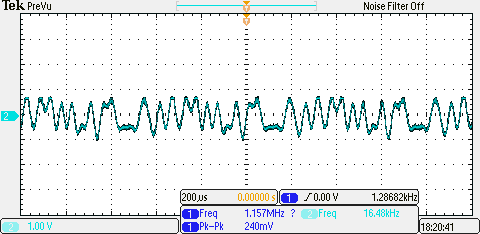
\includegraphics[width=0.65\textwidth]{img/periodic_pseudo_sequence}
    \caption{SSRG $[5,2]_s$.}
  \end{center}
\end{figure}

% PLACE HOLDER IMAGE FIGURE 1 SSRG [5,2]s.
%\begin{figure}[h]
%  \begin{center}
%    
\includegraphics[width=0.65\textwidth]{img/placeholder.jpg}
%    \caption{SSRG $[5,2]_s$.}
%  \end{center}
%\end{figure}

% count state table
\begin{center}
\begin{tabular}{c|c}
count & state \\ \hline
[0] & 10000 \\ \hline
[1] & 01000 \\ \hline
[2] & 10100 \\ \hline
[3] & 01010 \\ \hline
[4] & 10101 \\ \hline
[5] & 11010 \\ \hline
[6] & 11101 \\ \hline
[7] & 01110 \\ \hline
[8] & 10111 \\ \hline
[9] & 11011 \\ \hline
[10] & 01101 \\ \hline
[11] & 00110 \\ \hline
[12] & 00011 \\ \hline
[13] & 10001 \\ \hline
[14] & 11000 \\ \hline
[15] & 11100 \\ \hline
[16] & 11110 \\ \hline
[17] & 11111 \\ \hline
[18] & 01111 \\ \hline
[19] & 00111 \\ \hline
[20] & 10011 \\ \hline
[21] & 11001 \\ \hline
\end{tabular}
\end{center}
\begin{center}
\begin{tabular}{c|c}
count & state \\ \hline
[22] & 01100 \\ \hline
[23] & 10110 \\ \hline
[24] & 01011 \\ \hline
[25] & 00101 \\ \hline
[26] & 10010 \\ \hline
[27] & 01001 \\ \hline
[28] & 00100 \\ \hline
[29] & 00010 \\ \hline
[30] & 00001 \\ \hline
[31] & 10000 \\ \hline
[32] & 01000 \\ \hline
[33] & 10100 \\ \hline
[34] & 01010 \\ \hline
[35] & 10101 \\ \hline
[36] & 11010 \\ \hline
[37] & 11101 \\ \hline
[38] & 01110 \\ \hline
[39] & 10111 \\ \hline
[40] & 11011 \\ \hline
[41] & 01101 \\ \hline
[42] & 00110 \\ \hline
[43] & 00011 \\ \hline
[44] & 10001 \\ \hline
[45] & 11000 \\ \hline
[46] & 11100 \\ \hline
[47] & 11110 \\ \hline
[48] & 11111 \\ \hline
[49] & 01111 \\ \hline
[50] & 00111 \\ \hline
[51] & 10011 \\ \hline
[52] & 11001 \\ \hline
[53] & 01100 \\ \hline
[54] & 10110 \\ \hline
[55] & 01011 \\ \hline
\end{tabular}
\end{center}
\begin{center}
\begin{tabular}{c|c}
count & state \\ \hline
[56] & 00101 \\ \hline
[57] & 10010 \\ \hline
[58] & 01001 \\ \hline
[59] & 00100 \\ \hline
[60] & 00010 \\ \hline
[61] & 00001 \\ \hline
[62] & 10000 \\ \hline
[63] & 01000 \\ \hline
[64] & 10100 \\ \hline
[65] & 01010 \\ \hline
[66] & 10101 \\ \hline
[67] & 11010 \\ \hline
[68] & 11101 \\ \hline
[69] & 01110 \\ \hline
[70] & 10111 \\ \hline
[71] & 11011 \\ \hline
[72] & 01101 \\ \hline
[73] & 00110 \\ \hline
[74] & 00011 \\ \hline
[75] & 10001 \\ \hline
[76] & 11000 \\ \hline
[77] & 11100 \\ \hline
[78] & 11110 \\ \hline
[79] & 11111 \\ \hline
[80] & 01111 \\ \hline
[81] & 00111 \\ \hline
[82] & 10011 \\ \hline
[83] & 11001 \\ \hline
[84] & 01100 \\ \hline
[85] & 10110 \\ \hline
[86] & 01011 \\ \hline
[87] & 00101 \\ \hline
[88] & 10010 \\ \hline
[90] & 01001 \\ \hline
[91] & 00100 \\ \hline
[92] & 00010 \\ \hline
[93] & 00001 \\ \hline
[94] & 10000 \\ \hline
[95] & 01000 \\ \hline
[96] & 10100 \\ \hline
[97] & 01010 \\ \hline
[98] & 10101 \\ \hline
[99] & 11010 \\ \hline

\end{tabular}
\end{center}


% PN sequence profiling
\begin{figure}[h]
  \begin{center}
    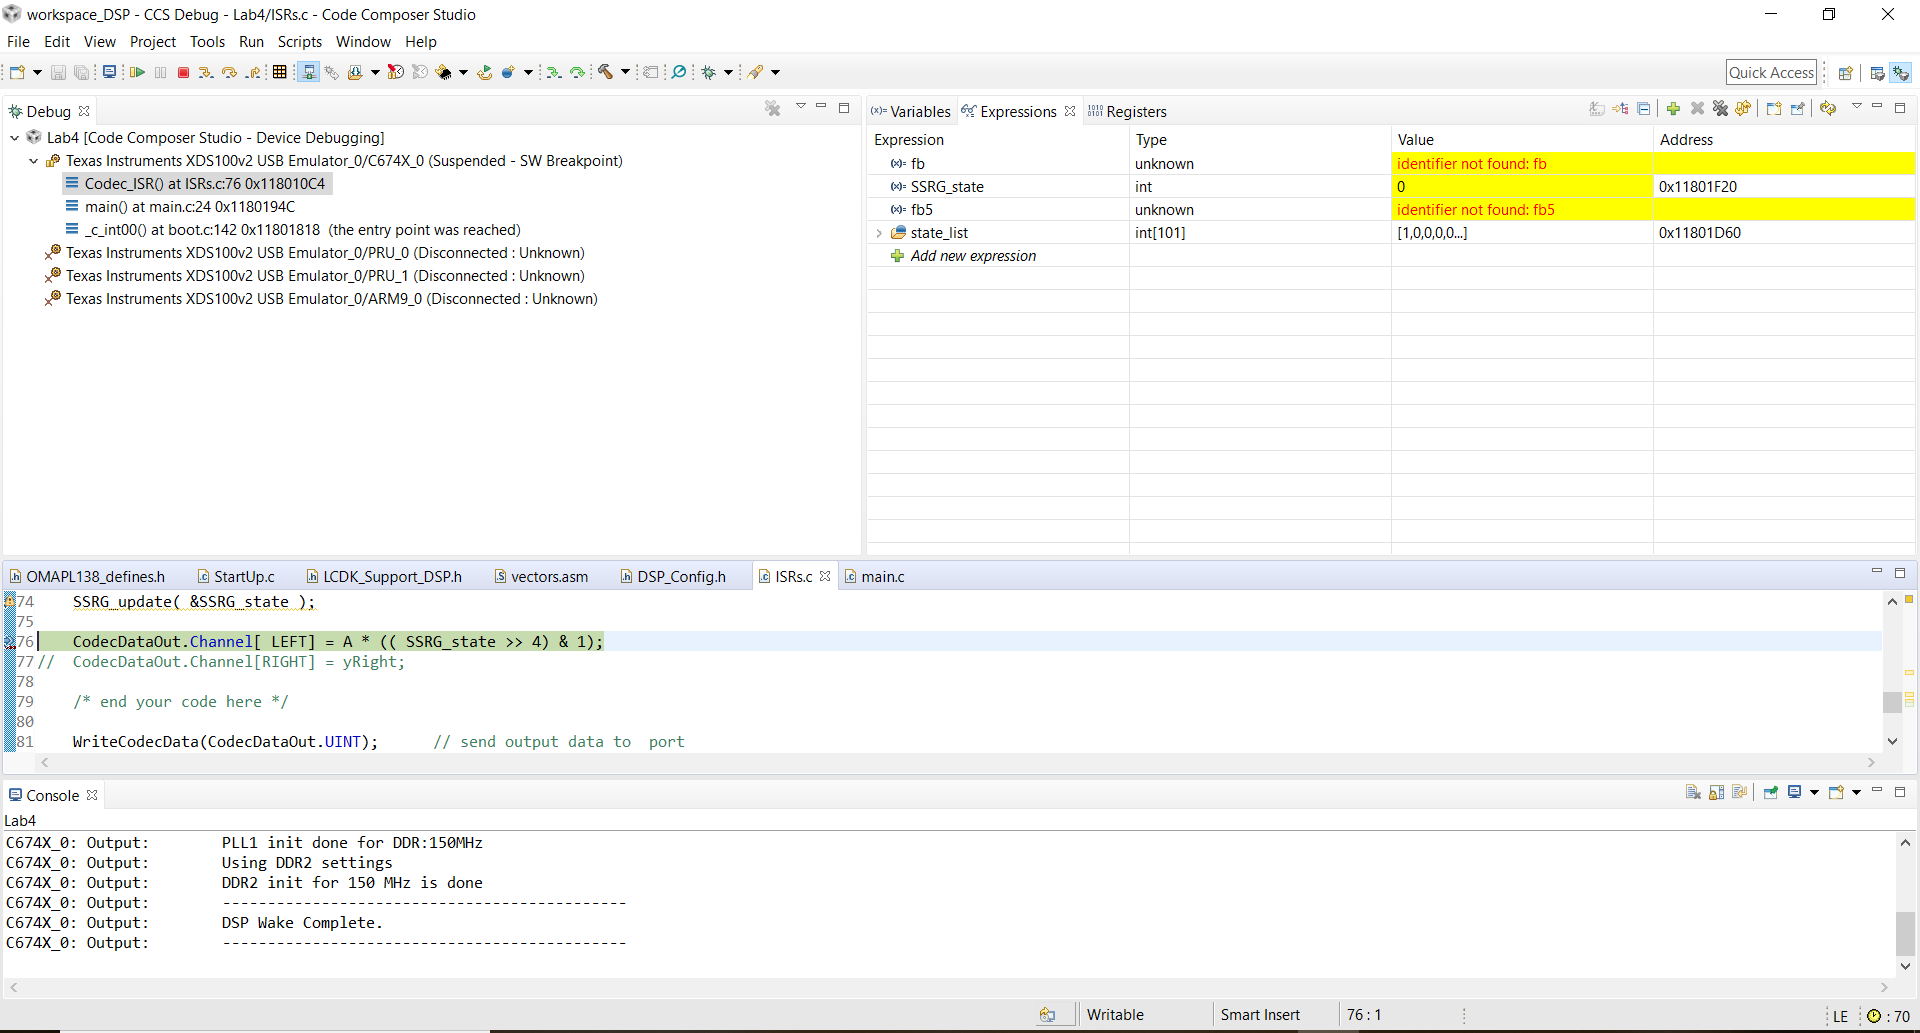
\includegraphics[width=0.65\textwidth]{img/profile_PN_generation.png}
    \caption{PN Sequence?.}
  \end{center}
\end{figure}


% PN generation C code 
\textbf{PN Generation C Code:}

\begin{verbatim}
\end{verbatim}

\subsection{DSK Implementation of Data Scrambler and Descrambler}
TODO

% count scrambler descrambler
\begin{center}
\begin{tabular}{c|c|c}
Count & Scrambler Output & Descrambler Output \\ \hline
[0] & 0 & 1 \\ \hline
[1] & 1 & 1 \\ \hline
[2] & 1 & 1 \\ \hline
[3] & 1 & 1 \\ \hline
[4] & 1 & 1 \\ \hline
[5] & 0 & 1 \\ \hline
[6] & 1 & 1 \\ \hline
[7] & 0 & 1 \\ \hline
[8] & 1 & 1 \\ \hline
[9] & 0 & 1 \\ \hline
[10] & 0 & 1 \\ \hline
[11] & 0 & 1 \\ \hline
[12] & 1 & 1 \\ \hline
[13] & 0 & 1 \\ \hline
[14] & 0 & 1 \\ \hline
[15] & 1 & 1 \\ \hline
[16] & 1 & 1 \\ \hline
[17] & 1 & 1 \\ \hline
[18] & 0 & 1 \\ \hline
[19] & 0 & 1 \\ \hline
[20] & 0 & 1 \\ \hline
[21] & 0 & 1 \\ \hline
\end{tabular}
\end{center}
\begin{center}
\begin{tabular}{c|c|c}
Count & Scrambler Output & Descrambler Output \\ \hline
[22] & 0 & 1 \\ \hline
[23] & 1 & 1 \\ \hline
[24] & 1 & 1 \\ \hline
[25] & 0 & 1 \\ \hline
[26] & 0 & 1 \\ \hline
[27] & 1 & 1 \\ \hline
[28] & 0 & 1 \\ \hline
[29] & 1 & 1 \\ \hline
[30] & 1 & 1 \\ \hline
[31] & 0 & 1 \\ \hline
[32] & 1 & 1 \\ \hline
[33] & 1 & 1 \\ \hline
[34] & 1 & 1 \\ \hline
[35] & 1 & 1 \\ \hline
[36] & 0 & 1 \\ \hline
[37] & 1 & 1 \\ \hline
[38] & 0 & 1 \\ \hline
[39] & 1 & 1 \\ \hline
[40] & 0 & 1 \\ \hline
[41] & 0 & 1 \\ \hline
[42] & 0 & 1 \\ \hline
[43] & 1 & 1 \\ \hline
[44] & 0 & 1 \\ \hline
[45] & 0 & 1 \\ \hline
[46] & 1 & 1 \\ \hline
[47] & 1 & 1 \\ \hline
[48] & 1 & 1 \\ \hline
[49] & 0 & 1 \\ \hline
[50] & 0 & 1 \\ \hline
[51] & 0 & 1 \\ \hline
[52] & 0 & 1 \\ \hline
[53] & 0 & 1 \\ \hline
[54] & 1 & 1 \\ \hline
[55] & 1 & 1 \\ \hline
\end{tabular}
\end{center}
\begin{center}
\begin{tabular}{c|c|c}
Count & Scrambler Output & Descrambler Output \\ \hline
[56] & 0 & 1 \\ \hline
[57] & 0 & 1 \\ \hline
[58] & 1 & 1 \\ \hline
[59] & 0 & 1 \\ \hline
[60] & 1 & 1 \\ \hline
[61] & 1 & 1 \\ \hline
[62] & 0 & 1 \\ \hline
[63] & 1 & 1 \\ \hline
[64] & 1 & 1 \\ \hline
[65] & 1 & 1 \\ \hline
[66] & 1 & 1 \\ \hline
[67] & 0 & 1 \\ \hline
[68] & 1 & 1 \\ \hline
[69] & 0 & 1 \\ \hline
[70] & 1 & 1 \\ \hline
[71] & 0 & 1 \\ \hline
[72] & 0 & 1 \\ \hline
[73] & 0 & 1 \\ \hline
[74] & 1 & 1 \\ \hline
[75] & 0 & 1 \\ \hline
[76] & 0 & 1 \\ \hline
[77] & 1 & 1 \\ \hline
[78] & 1 & 1 \\ \hline
[79] & 1 & 1 \\ \hline
[80] & 0 & 1 \\ \hline
[81] & 0 & 1 \\ \hline
[82] & 0 & 1 \\ \hline
[83] & 0 & 1 \\ \hline
[83] & 0 & 1 \\ \hline
[84] & 1 & 1 \\ \hline
[85] & 1 & 1 \\ \hline
[86] & 0 & 1 \\ \hline
[87] & 0 & 1 \\ \hline
[88] & 1 & 1 \\ \hline
[89] & 0 & 1 \\ \hline
[90] & 1 & 1 \\ \hline
[91] & 1 & 1 \\ \hline
[92] & 0 & 1 \\ \hline
[93] & 1 & 1 \\ \hline
[94] & 1 & 1 \\ \hline
[95] & 1 & 1 \\ \hline
[96] & 1 & 1 \\ \hline
[97] & 0 & 1 \\ \hline
[98] & 1 & 1 \\ \hline
[99] & 0 & 1 \\ \hline

\end{tabular}
\end{center}

% Scrambler and Descrambler profiling
\begin{figure}[h]
  \begin{center}
    
\includegraphics[width=0.65\textwidth]{img/placeholder.jpg}
    \caption{Scrambler and Descrambler Profiling}
  \end{center}
\end{figure}


% scrambler and descrambler code 
\textbf{Scrambler and Descrambler C Code:}

\begin{verbatim}
\end{verbatim}

\subsection{Autocorrelation}
TODO

% autocorelation code 
\textbf{Autocorrelation Code:}

\begin{verbatim}
\end{verbatim}

% IMAGE PN Circular autocorrelation
\begin{figure}[h]
  \begin{center}
    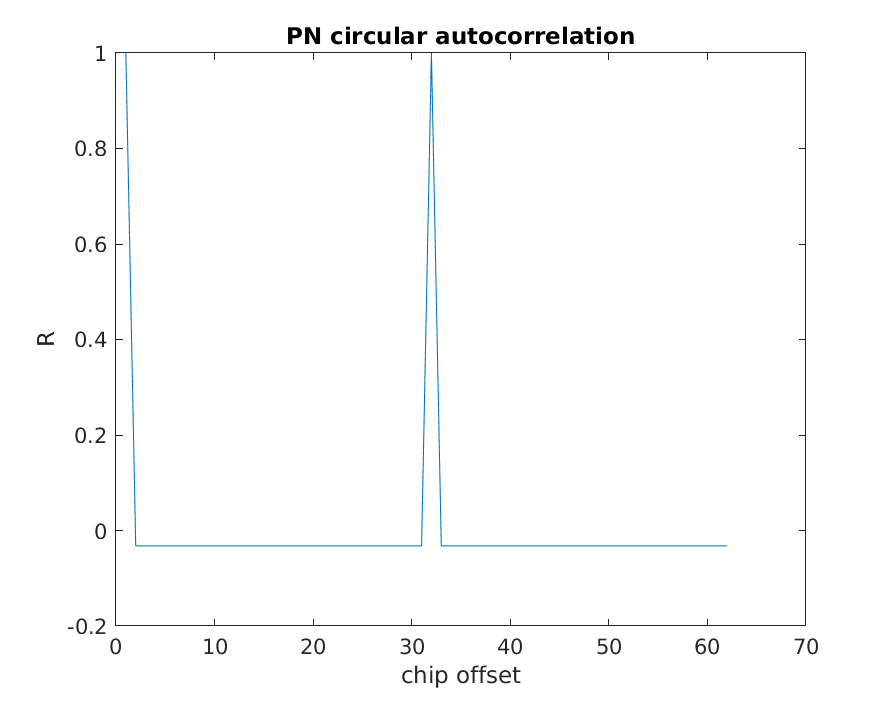
\includegraphics[width=0.65\textwidth]{img/pn_corr.png}
    \caption{PN Sequence Autocorrelation.}
  \end{center}
\end{figure}
% IMAGE Scrambled circular autocorrelation
\begin{figure}[h]
  \begin{center}
    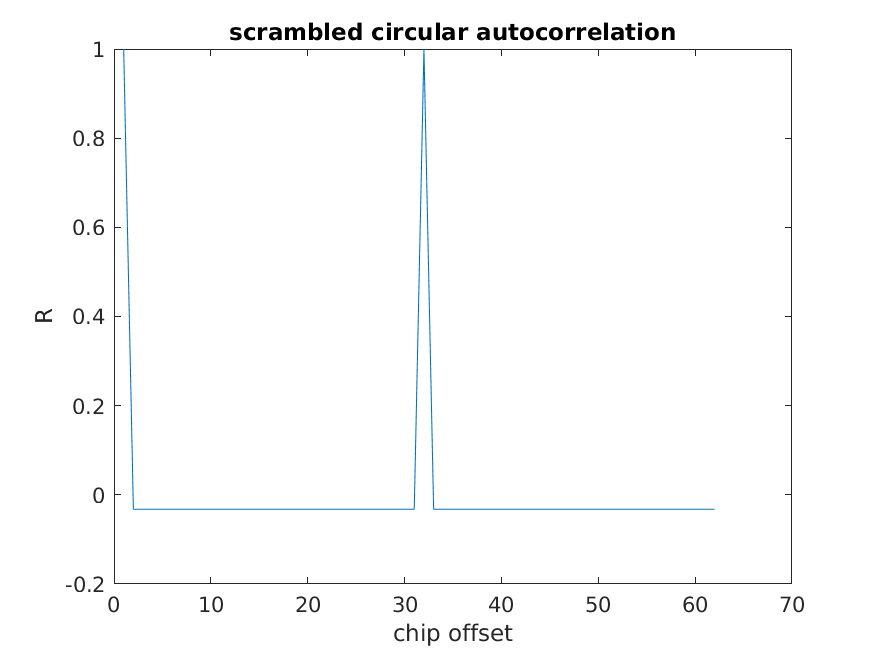
\includegraphics[width=0.65\textwidth]{img/sc_corr.png}
    \caption{Scrambler Autocorrelation.}
  \end{center}
\end{figure}


%----------------------------------------------------------------------------------------
%	SECTION 4
%----------------------------------------------------------------------------------------

\section{Discussion}

\subsection{TODO}


%----------------------------------------------------------------------------------------
%	SECTION 5
%----------------------------------------------------------------------------------------

\section{Answers to questions}

\begin{enumerate}
  \begin{item}
    Number of taps before you run out of time for FIR filtering.

  \textbf{Answer:}

\end{enumerate}

%----------------------------------------------------------------------------------------
%	BIBLIOGRAPHY
%----------------------------------------------------------------------------------------

\bibliography{mybib}
\bibliographystyle{plain}

%----------------------------------------------------------------------------------------


\end{document}
